\documentclass[a4paper,11pt]{report}
\usepackage[]{amsmath}
\usepackage[]{physics} % \bra, \ket etc
\usepackage{graphicx} %Pour les figures je crois
\usepackage{hyperref}
\usepackage[
    backend=biber, 
    natbib=true,
    style=numeric,
    sorting=none, %Pour faire apparaitre les refs dans l'ordre
    hyperref=true
]{biblatex} %Imports biblatex package
\addbibresource{Bib_ch3.bib} %Import the bibliography file

\usepackage{amssymb} %quelques symboles dont gtrsim /lesssim
\usepackage{subcaption} % package pour faire des subfigures
\usepackage{multirow} % package pour multirow/multicolumn
\usepackage{booktabs} % package pour top/mid/bottom rule
\usepackage{tcolorbox} % toujours plus de boites
\usepackage{xcolor} % Pour avoir des couleurs dans les équations

\title{}
\begin{document}
\chapter{NV-NV cross-relaxations : the fluctuator model}
In this chapter,...



\section{Experimental observation of NV-NV cross-relaxation}
Before we discuss the theoretical complications related to NV-NV cross-relaxations (CR), let us first show the unambiguous experimental proof of the presence of NV-NV CR.
\subsection{NV-NV CR between nonequivalent NV centers}
\begin{figure}[h]
\centering
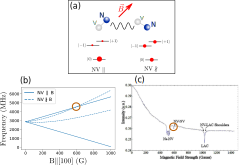
\includegraphics[width=\textwidth]{Figures/NV-NV_non_equivalent}[h]
\caption{label. Taken from \citep{armstrong2010nv}}
\label{non equivalent NV-NV}
\end{figure}
NV-NV CR was first observed more than thirty years ago \citep{holliday1989optical, van1989cross}. The first observations were between non-equivalent NV centers, meaning that the two NV centers involved in the dipole-dipole coupling were not polarized equally.

This scenario can happen for instance when two NV centers from different classes see a different transverse (and longitudinal) magnetic field. Fig \ref{non equivalent NV-NV} illustrates this in the case where the magnetic field is parallel with one of the four classes: $\mathbf{B} \parallel [111]$

When $\mathbf{B} \parallel [111]$, as we discussed in the last chapter, one class sees no transverse field and is therefore always polarized. The three other (equivalent) classes on the other hand get more and more depolarized as the magnetic field amplitude is increased. 

It turns out that there is a co-resonnance at B=592 G between the class parallel to $\mathbf{B}$ and the three other classes. This co-resonance is represented in Fig. \ref{non equivalent NV-NV}-b) by an orange circle.

Fig. \ref{non equivalent NV-NV}-c), which we already saw in the last chapter, shows the change in PL of an ensemble of NV centers as $\mathbf{B}$ is scanned along the [111] axis. For B=592 G, we can see a drop in PL also circled in orange. This drop is the result of the CR between NV centers from the class parallel to $\mathbf{B}$ and NV centers from the three other classes. 

While a difference in polarization is needed to observe a population transfer, it is not enough to explain the drop in PL. This PL drop is due to the difference in brightness between the $\ket{0}$ and $\ket{+1}$ from the different classes involved. The PL contrast between the two states is higher for the class parallel to $\mathbf{B}$ than for the three other ones, which is another consequence of the transverse field.

The co-resonance between two different classes of NV centers with different magnetic field projection is a relatively rare event: it can only occur for the $\ket{0} \to \ket{+1}$ transition, and only for magnetic fields greater than 592 G.

%techniquement y'a les resonances 0->-1 et -1/+1 mais c'est le delbor, j'ai pas envie d'embrouiller plus que ca.

\section{Microscopic origin of the fluctuators}
\subsection{Tunneling}
\subsection{Modulation of the J-coupling by the phonons}
"Electron Spin-Lattice Relaxation in Phosphorus-Doped Silicon"

"On the interaction of nuclear spins in a crystalline lattice"

"Concentration- and Compensation-Dependent Spin-Lattice Relaxation in n-Type Silicon"


Attention quand même, ce process dépend e la température si je dis pas de bêtises, c'est p-e pas ça chez nous. Nan ok, ça modifie gammaf mais pas le T1 directement. P-e que c'est mesurable ?

Attention bis : C'est l'exchange interaction (le terme en delta) qui est modifié, visiblement le couplage dipolaire etr trop faible pour expliquer ça (papier de Pines et "Spin Resonance of Impurity Atoms in Silicon"
\printbibliography
\end{document}